
\chapter{Place Value and Decimals}



\section{Review of Dots \& Boxes Model}\label{sec: review}
Let's start with a quick review of place value, different bases, and our ``Dots \& Boxes'' model for thinking about these ideas.

\begin{quote}
{\bf The $1 \leftarrow 2$ Rule (Base 2):\\
Whenever there are two dots in single box, they ``explode,'' disappear, and become one dot in the box to the left.}
\end{quote}

\bigskip

\begin{example}[Nine Dots in the $1 \leftarrow 2$ System]
We start by placing nine dots in the rightmost box.

\begin{center}
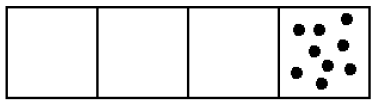
\includegraphics[height=1.5cm]{9dots1}
\end{center}
Two dots in that box explode and become one dot in the box to the left.
\begin{center}
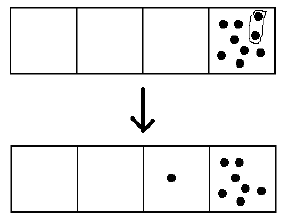
\includegraphics[height=4.5cm]{9dots2}
\end{center}
Since there are more than two dots in the rightmost box, it can happen again.
\begin{center}
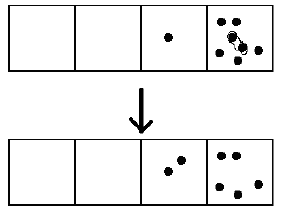
\includegraphics[height=4.5cm]{9dots3}
\end{center}
And again!
\begin{center}
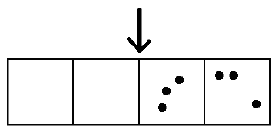
\includegraphics[height=3cm]{9dots4}
\end{center}
Now we have more than two dots in the second box, so those can explode and move!
\begin{center}
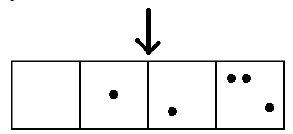
\includegraphics[height=3cm]{9dots5}
\end{center}
And the rightmost box still has more than two dots.
\begin{center}
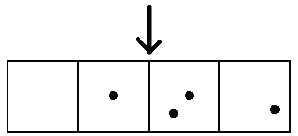
\includegraphics[height=3cm]{9dots6}
\end{center}
Keep going, until no box has two dots.
\begin{center}
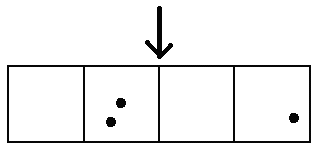
\includegraphics[height=3cm]{9dots7}

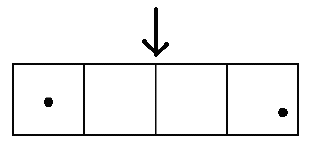
\includegraphics[height=3cm]{9dots8}
\end{center}
After all this, reading from left to right we are left with one dot, followed by zero
dots, zero dots, and one final dot.   This process lets us write the number of dots (nine) as a base-two or binary number:

\[
9_\text{ten} = 1001_\text{two}
\]
\end{example}


\bigskip
\bigskip


\begin{quote}
{\bf The $1 \leftarrow 3$ Rule (Base 3):\\
Whenever there are three dots in single box, they ``explode,'' disappear, and become one dot in the box to the left.}
\end{quote}

\begin{example}[Fifteen Dots in the $1 \leftarrow 3$ System]
Here's what happens with fifteen dots:
\begin{center}
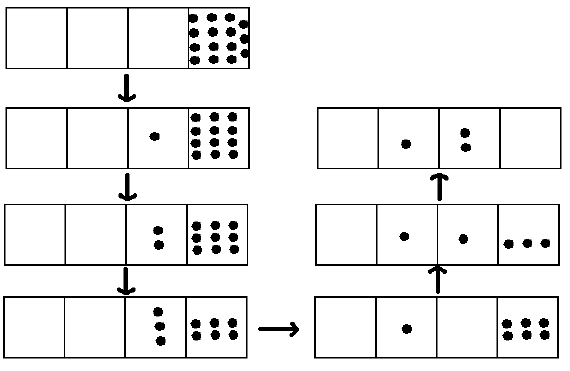
\includegraphics[height=8cm]{15dots}
\end{center}

Here's how we write fifteen in base 3:
\[
15_\text{ten} = 120_\text{three}.
\]

\end{example}


\bigskip
\bigskip

\begin{thinkpair*}
Work through the two  examples above carefully to be sure you remember and understand how the ``Dots \& Boxes'' model works.  Then answer these questions:
\begin{itemize}
\item
 When we write 9 in base 2, why do we write $1001_\text{two}$ instead of just $11_\text{two}$?\\
 \item
 When we write 15 in base 3, why do we write $120_\text{three}$ instead of just $12_\text{three}$?\\
 \item
 How many different \emph{digits} do you need in a base 7 system?  In a base 12 system?  In a base $b$ system?  How do you know?
 \end{itemize}
\end{thinkpair*}


\bigskip
\bigskip

\subsection*{On Your Own}
 Work on the following exercises on your own or with a partner.


\begin{enumerate}
\item
In base 4, four dots in one box are worth one dot in the box one place
to the left. 
\begin{enumerate}[(a)]
\item
What is the value of each box?
\begin{center}
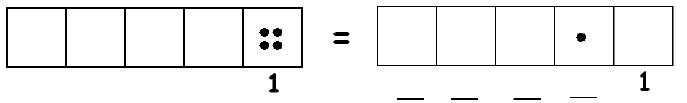
\includegraphics[height=2cm]{base4system}\\
\end{center}

\item
How do you write $29_\text{ten}$ in base 4?\\

\item
How do you write $132_\text{four}$ in base 10?\\
\end{enumerate}

\bigskip

\item
In our familiar base 10 system, ten dots in one box are worth one dot in the box one place
to the left. 
\begin{enumerate}[(a)]
\item
What is the value of each box?
\begin{center}
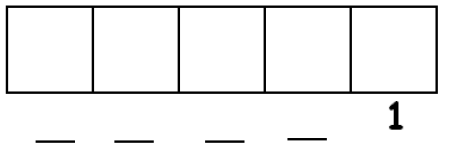
\includegraphics[height=2cm]{base10system}\\
\end{center}

\item
When we write the number 7842, what quantity does the  ``7'' represent? The ``4'' is
four groups of what value? The ``8'' is eight groups of what value? The ``2'' is two
groups of what value?\\

\end{enumerate}

\bigskip

\item
Write the following numbers of dots in base 2, base 3, base 5, and base 8.  Draw the ``Dots \& Boxes'' model if it helps you remember how to do this!  (Note: these numbers are all written in base 10.  When we don't say otherwise, you should assume base 10.)

\begin{center}
\begin{tabular}{l l}
(a) 2
\qquad\qquad
&(b) 17\\
\\
(c)
27
\qquad\qquad
&(d) 63
\end{tabular}\\
\end{center}

\bigskip

\item
Convert these numbers to our more familiar base ten system.  Draw out dots and boxes and ``unexplode'' the dots if it helps you remember!

\begin{center}

\begin{tabular}{l l}
(a) $1101_\text{two}$
\qquad\qquad
&(b) $102_\text{three}$\\
\\
(c)
$24_\text{five}$
\qquad\qquad
&(d) 
$24_\text{nine}$
\end{tabular}\\
\end{center}



\end{enumerate}

\bigskip
\bigskip


\begin{thinkpair*}
Quickly compute each of the following.  Write your answer in the same base as the problem.
\begin{itemize}
\item
$131_\text{ten} \text{ times ten}$\\
\item
 $263207_\text{eight} \text{ times eight}$\\
\item
$563872_\text{nine} \text{ times nine}$\\
\item
Use the $1 \leftarrow 10$ system to explain why multiplying a whole number in base 10 by 10 results in simply appending a zero to the right end of the number.\\

\item
Suppose you have a whole number written in base $b$.  What is the effect of multiplying that number  by $b$?  Justify what you say.

\end{itemize}

\end{thinkpair*}



\newpage




\section{Decimals}
Up to now our ``Dots \& Boxes'' model has consisted of a row of boxes extending infinitely far to the left. Why not have boxes extending to the right as well?

 

Let's work specifically with a  $1\leftarrow10$ rule and see what boxes to the right could mean.

 

\begin{center}
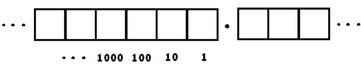
\includegraphics[height=2cm]{decimalsystem1}
\end{center}

\noindent
{\bf Notation:} It has become convention to separate boxes to the left from the ones to the right with a decimal point. (At least, this is what the point is called in the base ten world!)

\bigskip
\bigskip


What is the value of the first box to the right of the decimal point? If we denote its value as $x$ , we have that ten $x$'s is equivalent to 1. (Remember, we are using a $1\leftarrow10$ rule.)\label{base10:what value}



\begin{center}
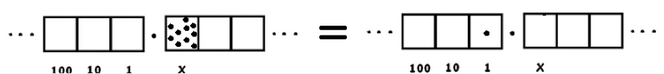
\includegraphics[height=1.75cm]{decimalsystem2}
\end{center}

\bigskip

From $10x=1$ we get that $x=\frac{1}{10}$.


\begin{center}
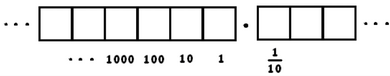
\includegraphics[height=2cm]{decimalsystem3}
\end{center}

\bigskip


Call the value of the next box to the right of the decimal point $y$.


\begin{center}
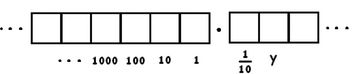
\includegraphics[height=2.3cm]{decimalsystem4}
\end{center}

From $10y=\frac1{10}$ we get $y=\frac1{100}$.

\bigskip
\bigskip
 

If we keep doing this, we see that the boxes to the right of the decimal point represent the reciprocals of the powers of ten.


\begin{center}
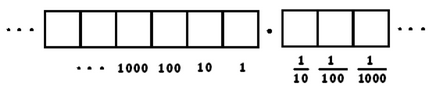
\includegraphics[height=2.25cm]{decimalsystem5}
\end{center}


\bigskip
\bigskip

\begin{example}[$0.3$ in Base Ten]
The decimal $0.3$ is represented by the picture:
\begin{center}
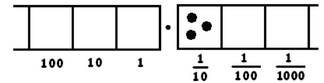
\includegraphics[height=2cm]{three-tenths}
\end{center}
It represents three groups of $\frac1{10}$, that is:
 \[
 0.3=\frac3{10}.
 \]

\end{example}



\bigskip
\bigskip



\begin{example}[$0.007$ in Base Ten]
The decimal $0.007$ is represented by the picture:
\begin{center}
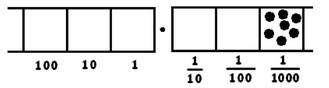
\includegraphics[height=2.25cm]{seven-thousandths}
\end{center}
It represents the fraction $\displaystyle\frac 7{1000}$.

\end{example}




\bigskip
\bigskip


Of course, some decimals represent fractions that can simplify (reduce) further. For example:

 

\[
0.5 
\ = \ 
\frac5{10}
\  = \ 
\frac12.
\]

 

Similarly, if a fraction can be rewritten to have a denominator that is a power of ten, then it is easy to convert it to a decimal. For example, $\frac 35$ is equivalent to $\frac 6{10}$ and so we have:

\[
\frac 35 
\ = \ 
 \frac6{10} 
 \ = \ 
0.6.
\]

 




\bigskip

\begin{example}[Decimal Representation of $12\frac 3 4$]
\label{example: dec 12 3/4}
Can you write $12\frac34$  as a decimal?
Well, 
\[
12\frac 34 \ =\ 12+\frac 34.
\]
 We can write the denominator as a power of ten using the key fraction rule:
 \[
 \frac 34 \cdot \frac{25}{25} 
 \ = \ 
 \frac{75}{100}.
 \]
 Thus we can now see that:
 \[
12\frac 34\ =\ 12+\frac{75}{100} \ = \ 12.75.
\]

\end{example}

\bigskip
\bigskip





\begin{thinkpair*}\ 
\begin{itemize}
\item
Draw a ``Dots \& Boxes'' picture for each of the following decimals.  Then say what fraction each decimal represents:  
\[
0.09   
\qquad\qquad
     0.003     
     \qquad\qquad
    0.7    
    \qquad\qquad
    0.0000003
    \]\
 

\item
Draw a ``Dots \& Boxes'' picture for each of the following fractions.  Then write the fraction as a decimal:  

 \[
\frac 1{1000}
    \qquad\qquad
   \frac 7{100}
       \qquad\qquad
      \frac9{10}
 \]\\
 
 \item
 What fractions (in simplest terms) do the following decimals represent?
 \[
 0.05   
     \qquad\qquad
      0.2       
          \qquad\qquad
       0.8      
           \qquad\qquad
         0.004
         \]\\
         
         \item
             Write the following fractions as decimals.
             \[
             \frac 25   
                 \qquad\qquad
    \frac 1{25}      
    \qquad\qquad
    \frac 1{20}      
    \qquad\qquad
    \frac 1{200}     
    \qquad\qquad
     \frac 1 {1250}
     \]\\
 

\item
Some people read $0.6$ out loud as ``point six.'' Others read it out loud as ``six tenths.'' 
Which is more helpful for understanding what the number really is? Why do you think so?

 \end{itemize}
 \end{thinkpair*}
 
 \bigskip
 
 
 \newpage
 
 \begin{example}[$0.31$ in Base Ten]\label{ex: 0.31 base 10}
 Here is a more interesting question:
What fraction is represented by the decimal $0.31$?

\begin{center}
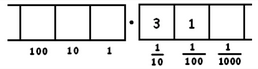
\includegraphics[height=2.25cm]{31-hundredths}
\end{center}


There are two ways to think about this.

\bigskip
\bigskip

 \begin{description}
 \item
 [Approach 1]   From the picture of the $1\leftarrow 10$ ``Dots \& Boxes'' model we see:  
 
 \[
 0.31\ =\ \frac 3{10}+\frac1{100}.
 \]
 
 \bigskip
 \bigskip
 \noindent
We can add these fractions by finding a common denominator:  

\[
\frac 3{10}+ \frac 1{100}\  =\ \frac {30}{100} +\frac 1{100}\ =\ \frac {31}{100}.
\]

\bigskip
 \bigskip
 \noindent
So 
\[
0.31
\ = \ 
\frac{31}{100}.
\]\\

 
\bigskip
\bigskip

\item[Approach 2]
Let's unexplode the three dots in the $\frac 1{10}$ position to produce an additional $30$ dots in the $\frac 1{100}$  position.

\begin{center}
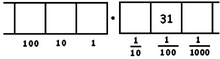
\includegraphics[height=2.25cm]{31-hundredths2}
\end{center}
So we can see right away that 
\[
0.31
\ = \ 
\frac{31}{100}.
\]\\
\end{description}
\end{example}

\newpage



\subsection*{On Your Own}
 Work on the following exercises on your own or with a partner.
 
 \begin{enumerate}
 
\item
 Brian is having difficulty seeing that $0.47$ represents the fraction $\frac{47}{100}$.  Describe the two approaches you could use to  explain this to him.\\
 
\item
A teacher asked his students to each draw a $1\leftarrow 10$ ``Dots \& Boxes'' picture of the fraction $\frac{319}{1000}$.
Jin drew this:
\begin{center}
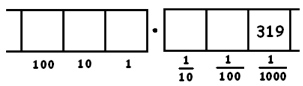
\includegraphics[height=2.5cm]{JinPic}
\end{center}
Sonia drew this:
\begin{center}
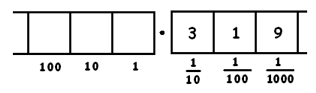
\includegraphics[height=2.6cm]{SoniaPic}
\end{center}
The teacher marked both students as correct. 
\begin{itemize}
\item
Are each of these solutions correct? Explain your thinking.\\
\item
Jin said he could get Sonia's solution by performing some explosions. What did he mean by this? Is he right?\\
\end{itemize}
 

\item
Choose the best answer and justify your choice. 
 The decimal $0.23$ equals:
 \begin{center}
\begin{align*}
(a)\  &\frac{23}{10}  
\qquad\qquad
  &(b)\  &\frac{23}{100}    \\
  \\
 (c) \ &\frac{23}{1000} 
 \qquad\qquad
   &(d)\   &\frac{23}{10000}
   \end{align*}\\
   
\end{center}
 
 \newpage

\item
Choose the best answer and justify your choice. 
The decimal $0.0409$ equals:
 \begin{center}
\begin{align*}
(a)\  &\frac{409}{100}
 \qquad\qquad
   &(b)\   &\frac{409}{1000} \\
   \\
  (c) \ &\frac{409}{10000} 
   \qquad\qquad
   &(d) \ &\frac{409}{100000}
   \end{align*}\\
 
\end{center}

\bigskip

\item
Choose the best answer and justify your choice. 
The decimal 0.050 equals:
 \begin{center}
\begin{align*}
(a) \  &\frac{50}{100}   
 \qquad\qquad
&(b) \  &\frac{1}{20  }\\
\\  (c)\ &\frac{1}{200} 
   \qquad\qquad
  &(d) \ &\text{None of these}
   \end{align*}\\
 
\end{center}

\bigskip
 

\item
Choose the best answer and justify your choice. 
  The decimal $0.000204$ equals
 \begin{center}
\begin{align*}
(a)\  &\frac{51}{250} 
   \qquad\qquad
   &(b) \  &\frac{51}{2500 }\\
\\
  (c)\ &\frac{ 51}{25000 } 
     \qquad\qquad
  &(d) \ &\frac{51}{250000}
   \end{align*}\\
 
\end{center}

\bigskip
 

 

\item
What fraction is represented by each of the following decimals?
\[
0.567       
     \qquad\qquad
0.031       
     \qquad\qquad
0.4077       
     \qquad\qquad
0.101
\]\\
 

\item
Write each of the following fractions as decimals.  Don't use a calculator!
\[
\frac{73}{100}         
 \qquad\qquad
\frac{519}{1000}
     \qquad\qquad
\frac{71}{1000}
     \qquad\qquad
\frac{7001}{10000}
 \]\\
 

\item
Write each of the following fractions as decimals.  Don't use a calculator!
\[
\frac{7}{20} 
     \qquad\qquad
     \frac{16}{25}   
          \qquad\qquad
 \frac{301}{500}      
      \qquad\qquad
\frac{17}{50}     
     \qquad\qquad
\frac{3}{4}
\]\\
 

 

 

\item
Write each of the following as a fraction (or mixed number).
\[
2.3 
     \qquad\qquad
 17.04     
  \qquad\qquad
 1003.1003 
 \]\\
 
 
 \item
 Write each of the following numbers in decimal notation:
 
 \[
5\frac{3}{10}
     \qquad\qquad
    7\frac15   
         \qquad\qquad
  13\frac12 
       \qquad\qquad
   106\frac3{20}
   \]\\
   
   \[
\frac{78}{25}       
     \qquad\qquad
\frac{9}{4}      
     \qquad\qquad
 \frac{131}{40}
\]\\

 

  \end{enumerate}


 
\newpage
 

Do $0.19$ and $0.190$ represent the same number or different numbers?
Here are two dots and boxes pictures for the decimal $0.19$.

\bigskip

\begin{center}
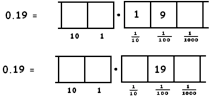
\includegraphics[height=4cm]{19-hundredths1}
\end{center}

\bigskip
\bigskip


And here are two dots and boxes picture for the decimal $0.190$.

\bigskip

\begin{center}
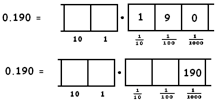
\includegraphics[height=4cm]{19-hundredths2}
\end{center}


\bigskip
\bigskip
\bigskip

\begin{thinkpair*}\ 
\begin{itemize}
\item
 Explain how one ``unexplosion'' establishes that the first picture of $0.19$ equivalent to the second picture of $0.19$.\\
 
 \item
     Explain how several unexplosions establishes that the first picture of $0.190$ equivalent to the second picture of $0.190$.\\
     
     \item
          Use explosions and unexplosions to show that all four pictures are equivalent to each other.\\
          
\item
So\dots does 0.190 represent the same number as 0.19?\\
\end{itemize}
\end{thinkpair*}

 \newpage
 

\section{$x$-mals}

Just like in base 10, we can add boxes to the right of the decimal point other bases, like base 5.  

\fellow{Add picture: dots and boxes for base five with 1's, 5's, 25's and 125's labeled.  Then a box to the right of the radix point with label $x$ and a box to the right of that labeled $y$, like on page 6.}


However, the prefix ``dec'' in ``decimal point'' means ten.  So we really shouldn't call it a decimal point anymore.  Maybe a ``pentimal point''?  In fact, the general term is ``radix point.''

\bigskip
\bigskip

\begin{thinkpair*}
Use reasoning like you saw on page~\ref{base10:what value} for the base ten system to think about other number systems:
\begin{itemize}
\item
 Figure out the values of $x$ and $y$ in the picture of the base-5 system above.    Be sure you can explain your reasoning.\\
 
 \item
 Draw a base-4 ``Dots \& Boxes'' model, including a radix point and some boxes to the right.  Label at least three boxes to the left of the ones place and three boxes to the right of the ones place.\\
 
 \item
 Draw a base-6 ``Dots \& Boxes'' model, including a radix point and some boxes to the right.  Label at least three boxes to the left of the ones place and three boxes to the right of the ones place.\\
 \end{itemize}


\end{thinkpair*}
 


\bigskip
\bigskip


In general, in a base-$b$ system, the boxes to the left of the ones place represent positive powers of the base $b$.  Boxes to the right of the ones place represent reciprocals of those powers.



\fellow{Add picture: dots and boxes for base $b$ with several boxes on each side labeled.}




\subsection*{On Your Own}
 Work on the following exercises on your own or with a partner.
 
 \begin{enumerate}
\item
Draw a ``Dots \& Boxes'' picture of each number:
\[
0.03_\text{five}
\qquad\qquad
0.22_\text{six}
\qquad\qquad
0.103_\text{four}
\qquad\qquad
0.002_\text{three}
\]\\

\item
Find a familiar (base-10) fraction value for each number:
\[
0.04_\text{five}
\qquad\qquad
0.3_\text{six}
\qquad\qquad
0.02_\text{four}
\qquad\qquad
0.03_\text{nine}
\]\\


\item
Find a familiar (base-10) fraction value for each number.  You might want to re-read Example~\ref{ex: 0.31 base 10} first!
\[
0.13_\text{five}
\qquad\quad
0.25_\text{six}
\qquad\quad
0.101_\text{two}
\qquad\quad
0.24_\text{seven}
\qquad\quad
0.55_\text{eight}
\]\\

\end{enumerate}


\bigskip
\bigskip

\begin{thinkpair*}
Tami and Courtney were working on converting $0.44_\text{five}$ to a familiar base-10 fraction.  Courtney said this:
\begin{quotation}
\emph{The places in base five to the right of the point are like $\frac 1 5$ and then $\frac 1{25}$.  Since this has two places, the answer should be $\frac{44}{25}$.}
\end{quotation}
\fellow{add picture of $0.44_\text{five}$ in a Dots \& Boxes model... four dots in each box.}

Tami thought about what Courtney said and replied:
\begin{quotation}
\emph{I don't know what the right answer is, but I know that $\frac{44}{25}$ can't be right.  The number $0.44_\textup{five}$ is less than one, since there are no numbers in the ones place and no explosions that we can do.  But the fraction $\frac{44}{25}$ is more than one.  It's almost two.  So they can't be the same number.}
\end{quotation}

\medskip

\begin{itemize}
\item
Who makes the most sense, Courtney or Tami?  Why do you think so?\\

\item
Find the right answer to the problem Courtney and Tami were working on.
\end{itemize}

\end{thinkpair*}

\bigskip
\bigskip


\begin{problem}
Find the ``decimal'' representation of  $\frac{1}{4} $ in each of the following bases.   Be sure that you can justify your answer.
\[
\text{base } 2
\qquad\quad
\text{base } 4
\qquad\quad
\text{base } 6
\qquad\quad
\text{base } 8
\qquad\quad
\text{base } 10
\qquad\quad
\text{base } 12
\]
\emph{Hint:  You might want to review Example~$\ref{example: dec 12 3/4}$.}
\end{problem}

\newpage


\section{Division and  Decimals}\label{sec: div & dec}
When you studied fractions, you had lots of different ways to think about them.  But the first way, and the one we keep coming back to, is   to think of a fraction as the answer to a division problem.  

\fellow{Throughout: pies per kid instead of pies per boy!}

\bigskip

\begin{example}[Pies per boy]
Suppose 6 pies are to be shared equally among 3 boys. This yields 2
pies per boy. We write:
\[
\frac 6 3 = 2.
\]


\begin{center}
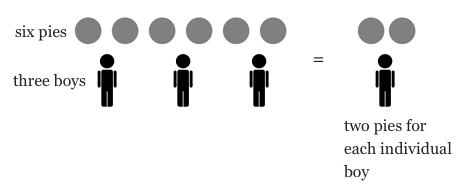
\includegraphics[height = 4.5cm]{PPB1}
\end{center}

The fraction $\frac 6 3$ is equivalent to the answer to the division problem $6 \div 3 = 2$.  It represents the number of pies one whole boy receives. 
\end{example}


\bigskip

\bigskip


In the same way \dots

\begin{itemize}
\item[]
sharing 10 pies among 2 boys yields $ \frac{10}2 = 5 $ pies per boy,\\
\item[]
sharing 8 pies among 2 boys yields $ \frac{8}2 = 4 $ pies per boy,\\
\item[]
sharing 5 pies among 5 boys yields $ \frac{5}5 = 1 $ pies per boy, and\\


\item[]
the answer to sharing 1 pies among 2 boys is $ \frac{1}2 $, which we call ``one-half.''


\end{itemize}



\begin{center}
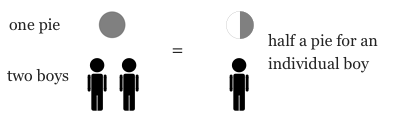
\includegraphics[height = 4cm]{PPB2}
\end{center}



We associate the number ``$\frac 1 2$'' to the picture

\includegraphics[height = 15pt]{halfpie}.

In the same way, the picture 
\includegraphics[height = 15pt]{thirdpie} represents ``one third,'' that is,
$ \frac 1 3$.
(This is  the amount of pie an individual boy would receive if one pie is
shared by three boys.)


The picture

\includegraphics[height = 15pt]{fifthpie}
 is called ``one fifth'' and is indeed
$\frac 1 5$, the amount of pie an
individual boy receives when one pie is shared among five.
 
And the picture
 
\includegraphics[height = 15pt]{3fifthpie}
 is called ``three fifths'' to represent
$\frac 3 5$,
the amount of pie
an individual receives if three pies are shared among five boys.

\bigskip
\bigskip

We know how to do division in our ``Dots \& Boxes'' model.  

\begin{example}[$3906 \div 3$]\label{ex: d&b divide1}
Suppose you are asked to compute $3906 \div 3$.  One way to interpret this question (there are others) is:
\begin{quote}
``How many groups of 3 fit into 3906?''
\end{quote}


In our ``Dots \& Boxes'' model, the dividend 3906 looks like this:
\begin{center}
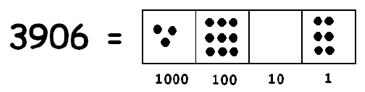
\includegraphics[height=2.5cm]{divide1}
\end{center}
and three dots looks like this:

\includegraphics[height=.4cm]{divide2}.
So we are really asking:

\begin{quote}
``How many groups of 
\includegraphics[height=.4cm]{divide2} fit into the picture of 3906?''
\end{quote}

There is  one group of 3 at the thousands level, and three at the hundreds level,
none at the tens level, and two at the ones level.
\begin{center}
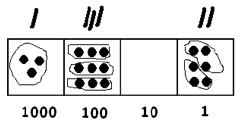
\includegraphics[height=3.25cm]{divide3}
\end{center}

Notice what we have in the picture:
\begin{itemize}
\item
One group of 3 in the thousands box.
\item
Three groups of 3 in the hundreds box.
\item
Zero groups of 3 in the tens box.
\item
Two groups of 3 in the ones box.
\end{itemize}
This shows that 3 goes into 3906 one thousand, three hundreds and two ones times. 
That is,
\[
3906 \div 3 = 1302.
\]
\end{example}

\bigskip
\bigskip

Of course, not every division problem works out evenly!  Here's a different example.

\begin{example}[$1024 \div 3$]\label{ex: divwithrem}
Suppose you are asked to compute $1024 \div 3$.  One way to interpret this question  is:
\begin{quote}
``How many groups of 3 fit into 1024?''
\end{quote}
So we're looking for groups of three dots in this picture:
\begin{center}
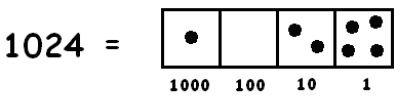
\includegraphics[height=2.25cm]{divide3a}
\end{center}
 One is
easy to spot:
 
 \begin{center}
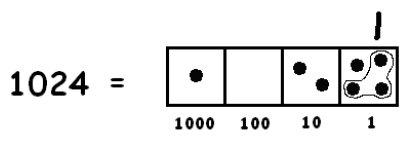
\includegraphics[height=3.25cm]{divide3b}
\end{center}
To find more groups of three dots, we must ``unexplode'' a dot:
 
 \begin{center}
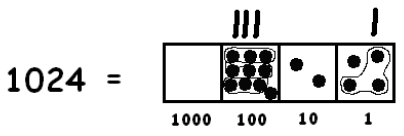
\includegraphics[height=3.25cm]{divide3c}
\end{center}
And we do it again:
 
 \begin{center}
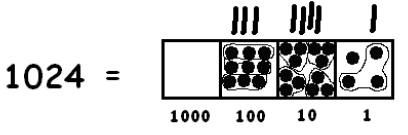
\includegraphics[height=3.25cm]{divide3d}
\end{center}
This leaves one stubborn dot remaining in the ones box and no more group of three. So we conclude:
\[
1024 \div 3 \ =\  341\  R 1.
\]

\end{example}


\bigskip
\bigskip
 
We can put these two ideas together --- fractions as the answer to a division problem and what we know about division in the ``Dots \& Boxes'' model ---   to help us think more about the connection between fractions and decimals.


\begin{example}[Decimal Representation of $\frac 1 8$]
The fraction $\frac 18$ is the result of dividing 1 by 8.
Let's actually compute $1\div 8$ in a $1\leftarrow 10$ ``Dots \& Boxes'' model, making use of decimals. We want to find groups of eight in the following picture:

\begin{center}
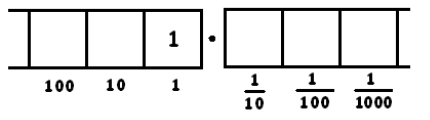
\includegraphics[height=3cm]{one-eighth1}
\end{center}
Clearly none are to be found, so let's unexplode:

\begin{center}
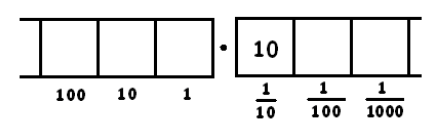
\includegraphics[height=3cm]{one-eighth2}
\end{center}


(We're being lazy and not drawing all the dots.  As you follow along, you might want to draw the dots rather than the number of dots, if it helps you keep track.)

 

Now there is one group of 8, leaving two behind.  We write a tick-mark on top, to keep track of the number of groups of 8, and leave two dots behind in the box.

\begin{center}
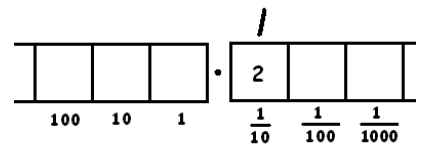
\includegraphics[height=3.5cm]{one-eighth3}
\end{center}
We can unexplode the two dots in the $\frac 1 {10}$ box:

\begin{center}
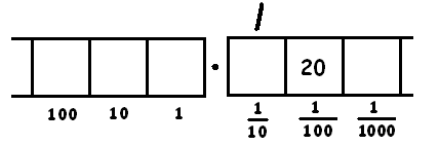
\includegraphics[height=3.5cm]{one-eighth4}
\end{center}
This gives two groups of 8 leaving four behind.  Remember: the two tick marks represent two groups of 8.  And there are four dots left in the box.

\begin{center}
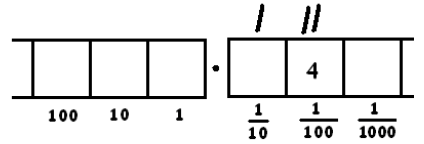
\includegraphics[height=3.2cm]{one-eighth5}
\end{center}
Unexploding those four remaining dots:

\begin{center}
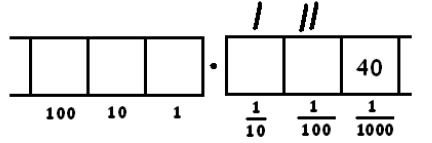
\includegraphics[height=3.2cm]{one-eighth6}
\end{center}
Now we have five groups of 8 and no remainder:

\begin{center}
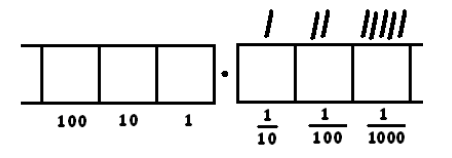
\includegraphics[height=3.5cm]{one-eighth7}
\end{center}

\newpage

Remember: the tick marks kept track of how many groups of eight there were in each box.  We have
\begin{itemize}
\item
One group of 8 dots in the $\displaystyle \frac 1 {10}$ box.\\
\item
Two groups of 8 dots in the $\displaystyle \frac 1{100}$ box.\\
\item
Five groups of 8 dots in the $\displaystyle \frac 1{1000}$ box.
\end{itemize}
So we conclude that
\[
 \frac 18
 \ = \ 
 1 \div 8 
 \ = \ 
 0.125.
 \]
Of course, it's a good habit to check our answer: 
\[
0.125
\ =\ 
\frac{125}{1000}
\ =\ 
\frac{\cancel{5}\cdot 25}{\cancel{5}\cdot 200}
\ =\ 
\frac{\cancel{5}\cdot 5}{\cancel{5}\cdot 40}
\ =\ 
\frac{\cancel{5}\cdot 1}{\cancel{5}\cdot 8}
\ =\ 
\frac 18.
\]
\end{example}


\bigskip
\bigskip

\subsection*{On Your Own}
 Work on the following exercises on your own or with a partner.  Be sure to show your work.
 
 \begin{enumerate}
 
\item
Perform the division in a $1\leftarrow 10$ ``Dots \& Boxes'' model to show that $\displaystyle \frac 14$, as a decimal, is $0.25$.\\

\item
Perform the division in a $1\leftarrow 10$ ``Dots \& Boxes'' model to show that $\displaystyle \frac 12$, as a decimal, is $0.5$.\\

\item
Perform the division in a $1\leftarrow 10$ ``Dots \& Boxes'' model to show that $\displaystyle \frac 35$, as a decimal, is $0.6$. \\

\item
Perform the division in a $1\leftarrow 10$ ``Dots \& Boxes'' model to show that $ \displaystyle\frac 3{16}$, as a decimal, is $0.1875$.\\
 
\item
 In simplest terms, what fraction is represented by each of these decimals?
\[
 0.75
\qquad\qquad
 0.625
\qquad\qquad
0.16
\qquad\qquad
0.85
\qquad\qquad
0.0625
\]
\end{enumerate}


\newpage

\subsection{Repeating Decimals}
Not all fractions lead to simple decimal representations. 

\begin{example}[Decimal Representation of $\frac 1 3$]
Consider the fraction $\frac 13$. We seek groups of three in the following picture:

\begin{center}
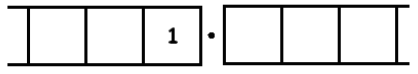
\includegraphics[height=1.9cm]{one-third1}
\end{center}
 

\noindent
Unexploding requires us to look for groups of 3 in:

\begin{center}
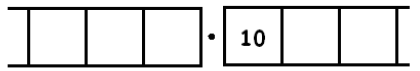
\includegraphics[height=1.9cm]{one-third2}
\end{center}
Here there are three groups of 3 leaving one behind:


\begin{center}
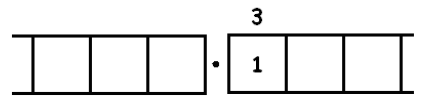
\includegraphics[height=2.8cm]{one-third3}
\end{center}
Unexploding gives:


\begin{center}
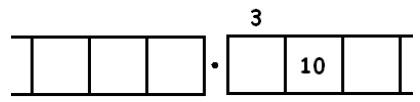
\includegraphics[height=2.8cm]{one-third4}
\end{center}
We find another three groups of 3 leaving one behind:


\begin{center}
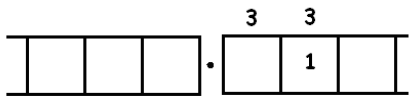
\includegraphics[height=2.8cm]{one-third5}
\end{center}

\newpage
\noindent
Unexploding gives:


\begin{center}
\includegraphics[height=2.8cm]{one-third6}
\includegraphics[height=3.1cm]{one-third7}
\end{center}
And\dots  we seem to be caught in an infinitely repeating cycle.
\end{example}

\bigskip
\bigskip

 

We are now in a philosophically interesting position. As human beings, we cannot conduct this, or any, activity  an infinite number of times. But it seems very tempting to write:

\[
\frac 13\ = \ 0.33333\dots,
\]
with the ellipsis ``\dots'' meaning  ``keep going forever with this pattern.''
We can \emph{imagine} what this means, but we  cannot actually \emph{write down} those infinitely many 3's represented by the \dots

 
 \bigskip
\bigskip

 
\noindent
{\bf Notation:} Many people make use of a \emph{vinculum} (horizontal bar) to represent infinitely long repeating decimals. For example,  $0.\bar3 $ means ``repeat the 3 forever'':
\[
0.\bar 3\ =\ 0.33333\dots,
\]
and $0.296\overline{412}$ means ``repeat 412 forever'':
\[
0.296\overline{412}\ = \ 0.296412412412412\dots
\]

 \bigskip
 \bigskip
 
 Now we're in a position to give a perhaps more satisfying answer to the question $1024 \div 3$.  In Example~\ref{ex: divwithrem}, we found the answer to be
 \[
 1024 \div 3 \ = \  341 \ R1.
 \]
 But now we know we can keep dividing that last stubborn dot by 3.  Remember, that $R1$ represents a single dot in the ones place, so if we keep dividing by three it really represents $\frac 1 3$.    So we have
  \[
 1024 \div 3 \ = \  341 \ R1
 \ = \ 
 341 \frac 1 3
  \ = \ 
341.333333\dots
 \]

 
 \bigskip
\bigskip
 
\begin{example}[Decimal Representation of $\frac 6 7$]
As another (more complicated) example, here is the work that converts the fraction $\frac 67$ to an infinitely long repeating decimal. Make sure to understand the steps one line to the next.

\bigskip

\includegraphics[height=3.5cm]{6-sevenths1}\\
\phantom{\quad} \includegraphics[height=4.2cm]{6-sevenths2}\\
\includegraphics[height=4.2cm]{6-sevenths3}\qquad\qquad\\
\qquad\includegraphics[height=4.2cm]{6-sevenths4}\\
 \includegraphics[height=4.25cm]{6-sevenths5}\\
\includegraphics[height=4.2cm]{6-sevenths6}\\
\includegraphics[height=2.5cm]{6-sevenths7}\
With this 6 in the final right-most box,  we have returned to the very beginning of the problem.  (Do you see why?  Remember, we started with a six in the ones box!)   

This means that we will simply repeat the work we have done and obtain the same sequence $857142$ of answers, and then again, and then again.
We have:
\begin{align*}
\frac 67 &\ =\ 0.857142857142857142857142\dots\\
&\ =\ 0.\overline{857142}.
\end{align*}
\end{example}

\bigskip
\bigskip



 \subsection*{On Your Own}
 Work on the following exercises on your own or with a partner.  Be sure to show your work.

\begin{enumerate}

\item
Compute $\displaystyle \frac 47$ as an infinitely long repeating decimal.\\

 

\item
  Compute $\displaystyle \frac 1{11}$ as an infinitely long repeating decimal.\\
  
  
  
\item
 Use a $1\leftarrow 10 $ ``Dots \& Boxes'' model to compute ${133}\div 6$.  Write the answer as a decimal. \\
 
\item
 Use a $1\leftarrow 10 $ ``Dots \& Boxes'' model to compute ${255}\div {11}$.  Write the answer as a decimal. \\
\end{enumerate}


\newpage

\section{More $x$-mals}

It should come as no surprise that we can use this reasoning about division in the ``Dots \& Boxes'' model in other bases as well. 
The following picture shows that working in base 5, 
\begin{equation}\label{eqn:base5div}
1423_\text{five}\div 13_\text{five}=110_\text{five}\ R2_\text{five}.
\end{equation}

\begin{center}
\includegraphics[height=2.75cm]{base5div0}
\end{center}

\begin{thinkpair*}
Carefully explain the connection between the picture and equation~\eqref{eqn:base5div} shown above.  
\begin{itemize}
\item
Show in the picture where you see $1423_\text{five}$ from the equation.\\
\item
 Where do you see $13_\text{five}$? \\
 \item
Where do you see $110_\text{five}$ and $2_\text{five}$?\\
\end{itemize}

\end{thinkpair*}


\bigskip


\begin{example}[$1423_\text{five}\div 13_\text{five}$]
Here is the (by now familiar) picture of base 5:
\begin{center}
\includegraphics[height=3cm]{base5div1}\
\end{center}

Now we can unexplode one of those two remaining dots.  Then we're able to make another group of  $13_\text{five}$.  
\begin{center}
\includegraphics[height=2.5cm]{base5div2}
\end{center}

Once again, there are two dots left over, not in any group.  So let's unexplode again.
\begin{center}
\includegraphics[height=2.5cm]{base5div3}
\end{center}

And we still have two dots left over.  Why not do it again?
\begin{center}
\includegraphics[height=2.25cm]{base5div4}
\end{center}

It seems like we're going to be doing the same thing forever:
\begin{itemize}
\item
Start with two dots  in some box.  \\
\item
Unexplode one one of the dots, so you have one dot in your original box and five in the box to the right.\\
\item
Form a group of $13_\text{five}$.  That uses the one dot in your original box and three of the five in the box to the right.\\
\item
So you have two dots left  in a  box.\\
\item
Unexplode one  of the dots, so you have one dot in your original box and five in the box to the right.\\
\item
This feels familiar\dots
\end{itemize}

\bigskip

We conclude:
\begin{equation}\label{eqn:base5div2}
1432_\text{five} \div 13_\text{five} = 110.111\dots_\text{five} = 110.\bar 1_\text{five}.
\end{equation}

 \end{example}
 
 \bigskip
 \bigskip
 
 \begin{thinkpair*} 
 Equation~\eqref{eqn:base5div2} is  a statement in base five.
What is it really saying? ``$1432_\text{five}$'' is the number 
\[
1\cdot 125+4\cdot 25+3\cdot 5+2\cdot 1=242_\text{ten}.
\]

 \begin{itemize}
 \item
 What is $13_\text{five}$ in base 10?  Be sure to  explain your answer.\\
 
 \item
 What is $110.\bar1_\text{five} $ in base 10?  Explain how you got your answer.\\
 
 \end{itemize}
 \end{thinkpair*}
 
 \bigskip
 \bigskip

\begin{problem}\ 
\begin{enumerate}[(a)]
\item
Draw the pictures to compute $8 \div 3$ in a base 10 system, and show the answer is $2.\bar6$.\\
\item
Draw the pictures to compute $8_\text{nine} \div 3_\text{nine}$ in a base 9 system, and write the answer as a decimal.  (Or is it a ``nonimal''?)\\
\end{enumerate}
\end{problem}

\bigskip

\begin{problem}\ 
\begin{enumerate}[(a)]
\item
Draw the pictures to compute $1 \div 11$ in a base 10 system, and show the answer is $0.\overline{09}$.\\

\item
Draw the base 3 pictures to compute $1_\text{three} \div 11_\text{three}$, and write the answer as a decimal (``trimal''?) number.\\

\item
Draw the base four pictures to compute $1_\text{four} \div 11_\text{four}$, and write the answer as a decimal (``quadimal''?) number.\\

\item
Draw the base six pictures to compute $1_\text{six} \div 11_\text{six}$, and write the answer as a decimal (``heximal''?) number.\\

\item
Describe any patterns you notice in the computations above.  Do you have a conjecture of a general rule?  Can you prove your general rule is true?
\end{enumerate}

\end{problem}


\bigskip
 

\begin{problem}
Remember that the fraction $\frac 2 5$ represents the division problem $2 \div 5$.  (This is all written in base 10.)
\begin{enumerate}[(a)]
\item
What is the decimal expansion (in base 10) of the fraction $\frac 2 5$?\\

\item
Rewrite the base-10 fraction $\frac 2 5$ as a base 4 division problem.  Then find the decimal expansion for that fraction in base 4.\\

\item
Rewrite the base-10 fraction $\frac 2 5$ as a base 5 division problem.  Then find the decimal expansion for that fraction in base 5.\\

\item
Rewrite the base-10 fraction $\frac 2 5$ as a base 7 division problem.  Then find the decimal expansion for that fraction in base 7.\\

\item
Barry said that in base 15, the division problem  looks like 
\[
2_\text{fifteen} \div 5_\text{fifteen},
\]
 and the decimal representation would be $0.6_\text{fifteen}$.  Check Barry's answer.  Is he right?

\end{enumerate}
\end{problem}







\begin{problem}\label{prob:1/b-1}
Expand each of the following as a ``decimal'' number in the base given.  (The fraction is given in base 10.)

\begin{align*}
(a) & \  \frac 1 9 \text{ in base } 10
&
(b) & \  \frac 1 2 \text{ in base } 3
\\
\\
(c) & \  \frac 1 3 \text{ in base } 4
&
(d) & \  \frac 1 4 \text{ in base } 5
\\
\\
(e) & \ \frac 1 5 \text{ in base } 6
& 
(f) & \ \frac 1 6 \text{ in base } 7
\\
\\
(g) & \  \frac 1 7 \text{ in base } 8
& 
(h) & \ \frac 1 8 \text{ in base } 9
\end{align*}


 \end{problem}

 


 \bigskip


\begin{problem}[{\bf Challenge}]
 What fraction has decimal expansion $0.\bar 3_\text{seven}$?  How do you know you are right?
  \end{problem}




\newpage

\section{Terminating or Repeating?}
You've seen that when you write a fraction as a decimal, sometimes the decimal \emph{terminates}, like
\[
\frac 1 2 = 0.5
\quad \text{ and } \quad
\frac {33} {1000} = 0.033.
\]
However, some fractions have  decimal representations that go on forever in a repeating pattern, like
\[
\frac 1 3 = 0.33333\dots
\quad \text{ and } \quad
\frac {6} {7} = 0.857142857142857142857142\dots.
\]
It's not totally obvious, but  it is true: those are the only two things that can happen when you write a fraction as a decimal.  

Of course, you can \emph{imagine} (but never write down) a fraction that goes on forever but doesn't repeat itself, for example:
\[
0.101001000100001000001\dots
\quad \text{ and } \quad
\pi = 3.14159265358979\dots
\]
But these numbers can never be written as a nice fraction $\frac a b$ where $a$ and $b$ are whole numbers.  They are  called \emph{irrational numbers}.  (The name does not indicate a judgement on their sanity.  Rather, fractions like $\frac a b$ are also called \emph{ratios}.  Irrational numbers cannot be expressed as a \emph{ratio} of two whole numbers.)

For now, we'll think about the question: Which fractions have decimal representations that terminate, and which fractions have decimal representations that repeat forever?  We'll focus just on \emph{unit fractions}.

\bigskip


\begin{define}
A \emph{unit fraction} is a fraction that has 1 in the numerator.  It looks like $\frac 1 n$ for some whole number $n$.
\end{define}

\bigskip



\begin{thinkpair*}\ 
\begin{itemize}
\item
 Which of the following fractions have infinitely long decimal representations and which do not?
\[
\frac 12 
\qquad
  \frac 13
  \qquad
   \frac 14 
   \qquad
  \frac15
  \qquad
   \frac16
\qquad
\frac 17 
\qquad
  \frac 18 
  \qquad
  \frac 19 
  \qquad
  \frac 1{10}
\]\\

\item
Try some more examples on your own.  Do you have a conjecture?
\begin{quote}
\emph{A fraction $\frac 1 b$ has an infinitely long decimal expansion if\\
\\
 \underline{\qquad\qquad\qquad\qquad\qquad\qquad\qquad\qquad\qquad\qquad\qquad}.}\\
\end{quote}
\end{itemize}
\end{thinkpair*}




\newpage

\begin{problem}\label{prob: powersof2}
 Complete the table below which shows the decimal expansion of unit fractions where the denominator is a power of 2.  (You may want to use a calculator to compute the decimal representations.  The point is to look for and then explain a pattern, rather than to compute by hand.)

\bigskip

\begin{center}
\begin{tabular}{ c | c  | c }
{\bf Fraction} & {\bf Denominator} & {\bf Decimal Representation} \\
\hline\hline
&&\\
$\displaystyle \frac 1 2$ & $2^1$ & $0.5$\\
&&\\
\hline
&&\\
$\displaystyle \frac 1 4$ & $2^2$ & $0.25$\\
&&\\
\hline
&&\\
$\displaystyle \frac 1 8$ & $2^3$ & $0.125$\\
&&\\
\hline
&&\\
$\displaystyle \frac 1 {16}$ &  &  \\
&&\\
\hline
&&\\
$\displaystyle \frac 1 {32}$ &  &  \\
&&\\
\hline
&&\\
$\displaystyle \frac 1 {64}$ &  &  \\
&&\\
\hline
&&\\
$\displaystyle \frac 1 {128}$ &  &  \\
&&\\
\hline
&&\\
$\displaystyle \frac 1 {256}$ &  &  \\
&&\\
\end{tabular}\\
\end{center}

\bigskip

\noindent
Try even more examples until you can make a conjecture:  What is the decimal representation of the unit fraction $\displaystyle \frac 1{2^n}$?  

\end{problem}

\newpage

\begin{problem}\label{prob: powersof5}
 Complete the table below which shows the decimal expansion of unit fractions where the denominator is a power of 5.  (You may want to use a calculator to compute the decimal representations.  The point is to look for and then explain a pattern, rather than to compute by hand.)

\bigskip

\begin{center}
\begin{tabular}{ c | c  | c }
{\bf Fraction} & {\bf Denominator} & {\bf Decimal Representation} \\
\hline\hline
&&\\
$\displaystyle \frac 1 5$ & $5^1$ & $0.2$\\
&&\\
\hline
&&\\
$\displaystyle \frac 1 {25}$ & $5^2$ & $0.04$\\
&&\\
\hline
&&\\
$\displaystyle \frac 1 {125}$ & $5^3$ & \\
&&\\
\hline
&&\\
$\displaystyle \frac 1 {625}$ &  &  \\
&&\\
\hline
&&\\
$\displaystyle \frac 1 {3125}$ &  &  \\
&&\\
\hline
&&\\
$\displaystyle \frac 1 {15625}$ &  &  \\
&&\\
\end{tabular}\\
\end{center}

\bigskip

\noindent
Try even more examples until you can make a general statement:  What is the decimal representation of the unit fraction $\displaystyle \frac 1{5^n}$?    


\end{problem}


\newpage

Marcus noticed a pattern in the table from Problem~\ref{prob: powersof2}, but was having trouble explaining exactly what he noticed.  Here's what he said to his group:

\begin{quote}
\emph{I remembered that when we wrote fractions as decimals before, we tried to make the denominator into a power of ten.  So we can do this:}
\begin{align*}
\frac 1 2 
\ &= \ 
\frac 1 2 \cdot \frac 5 5 
\ = \ 
\frac {5}{10}
\ = \ 
0.5\\
\\
\frac 1 4 
\ &= \ 
\frac 1 4 \cdot \frac {25}{25} 
\ = \ 
\frac {25}{100}
\ = \ 
0.25\\
\\
\frac 1 8 
\ &= \ 
\frac 1 8 \cdot \frac {125}{125} 
\ = \ 
\frac {125}{1000}
\ = \ 
0.125\end{align*}
\emph{When we only have $2$'s, we can always turn them into $10$'s by adding enough $5$'s.}
\end{quote}

\bigskip
\bigskip
\bigskip


\begin{thinkpair*}\ 
\begin{itemize}
\item
Write out several more examples of what Marcus discovered.\\

\item
If Marcus had the unit fraction $\frac1{2^n}$, what would be his first step to turn it into a decimal?  What would the decimal expansion look like and why?\\

\item
Now think about unit fractions with powers of 5 in the denominator.
If Marcus had the unit fraction $\frac1{5^n}$, what would be his first step to turn it into a decimal?  What would the decimal expansion look like and why?

\end{itemize}
\end{thinkpair*}

\newpage


\begin{problem}\label{prob: 2^nanswer}
Marcus has a really good insight, but he didn't explain it very well.   He doesn't really mean  that we ``turn 2's into 10's.'' And he's not doing any addition, so talking about ``adding enough 5's'' is pretty confusing.  

\begin{enumerate}[(a)]
\item
Complete the statement below by filling in the numerator of the fraction.  \begin{quote}
The unit fraction $\frac 1 {2^n}$ has a decimal representation that terminates.  The representation will have $n$ decimal digits, and will be equivalent to the fraction 
\[
\frac{?}{10^n}.
\]\\
\end{quote}

\item
Write a better version of Marcus's explanation to justify why this fact is true.
\end{enumerate}
\end{problem}

\bigskip
\bigskip

\begin{problem}
  Write a statement about the decimal representations of  unit fractions $\frac 1 {5^n}$ and justify that your statement is correct.
  (Use the statement in Problem~\ref{prob: 2^nanswer} as a model.)
\end{problem}


\bigskip
\bigskip

\begin{problem}
Each of the fractions listed below has a terminating decimal representation.  Explain how you could know this for sure, without actually calculating the decimal representation.
\[
\frac 1{10}
\qquad\quad
\frac 1{20}
\qquad\quad
\frac 1{50}
\qquad\quad
\frac 1{200}
\qquad\quad
\frac 1{500}
\qquad\quad
\frac 1{4000}
\]
\end{problem}



\newpage

\subsection{The period of a repeating decimal}
If the denominator of a fraction can be factored into just 2's and 5's, you can always form an equivalent fraction where the denominator is a power of ten.  For example, if we start with the fraction
\[
\frac 1 {2^a 5^b},
\]
we can form an equivalent fraction
\[
\frac 1 {2^a 5^b}
\ = \ 
\frac 1 {2^a 5^b} \cdot \frac {2^b 5^a} {2^b 5^a}
\ = \ 
\frac {2^b 5^a} {2^{a+b} 5^{a+b}}
\ = \ 
\frac {2^b 5^a} {10^{a+b}}.
\]
The denominator is a power of ten, so the decimal expansion is finite with (at most) $a+b$ places.


\bigskip

What about fractions where the denominator has other prime factors besides 2's and 5's?  Certainly we \emph{can't} turn the denominator into a power of 10, because powers of 10 have just 2's and 5's as their prime factors.  So in this case the decimal expansion will go on forever.  But why will it have a \emph{repeating pattern}?  And is there anything else interesting we can say in this case?
 

\bigskip
\bigskip

\begin{define}
The \emph{period} of a repeating decimal is the smallest number of digits that repeat.
\end{define}


\bigskip
\bigskip



For example, we saw that 
\begin{align*}
\frac 1 3 
&\ = \ 
0.33333\dots\\
&\ = \ 
0.\bar 3.
\end{align*}
The repeating part is just the single digit 3, so the period of this repeating decimal is one.

\bigskip


Similarly, we know that
\begin{align*}
\frac 67
&\ =\ 
0.857142857142857142857142\dots\\
&\ = \ 
0.\overline{857142}.
\end{align*}
The smallest repeating part is the digits $847142$, so the period of this repeating decimal is 6.

\bigskip

You can think of it this way: the \emph{period} is the length of the string of digits under the vinculum (the horizontal bar that indicates the repeating digits).


\newpage

\begin{problem}
 Complete the table below which shows the decimal expansion of unit fractions where the denominator has prime factors besides 2 and 5.   (You may want to use a calculator to compute the decimal representations.  The point is to look for and then explain a pattern, rather than to compute by hand.)

\bigskip

\begin{center}
\begin{tabular}{ c | c  | c }
{\bf Fraction} & {\bf Decimal Representation} & {\bf Period} \\
\hline\hline
&&\\
$\displaystyle \frac 1 3$ & $0.\bar 3$  &  1 \\
&&\\
\hline
&&\\
$\displaystyle \frac 1 6$ & $0.1\overline{6}$ & 1\\
&&\\
\hline
&&\\
$\displaystyle \frac 1 7$ & $0.\overline{142857}$ & 6\\
&&\\
\hline
&&\\
$\displaystyle \frac 1 {9}$ &  &  \\
&&\\
\hline
&&\\
$\displaystyle \frac 1 {11}$ &  &  \\
&&\\
\hline
&&\\
$\displaystyle \frac 1 {12}$ &  &  \\
&&\\
\hline
&&\\
$\displaystyle \frac 1 {13}$ &  &  \\
&&\\
\hline
&&\\
$\displaystyle \frac 1 {14}$ &  &  \\
&&\\
\end{tabular}\\
\end{center}

\bigskip

\noindent
Try even more examples until you can make a conjecture:  What can you say about the period of the fraction $\frac 1 n$ when $n$ has prime factors besides 2 and 5?
\end{problem}


\newpage



Imagine you are doing the ``Dots \& Boxes'' division to compute the decimal representation of a unit fraction like $\frac 1 6$.  You start with a single dot  in the ones box:

\begin{center}
\includegraphics[height=3cm]{one-eighth1}
\end{center}

\bigskip
\noindent
To find the decimal expansion, you  ``unexplode'' dots, form groups of six, see how many dots are left, and repeat.
 
 \bigskip
 \bigskip
 
Draw your own pictures to follow along this explanation:
\begin{itemize}
\item
When you unexplode the first dot, you get 10 dots in the $\frac 1{10}$ box, which gives one group of six
 with remainder of 4.\\

\item
When you unexplode those four dots, you get 40 dots in the $\frac 1{100}$ box, which gives six group of six
 with remainder of 4.\\
 \end{itemize}
 
 Since the remainder repeated (we got a remainder of 4 again), we can see that the process will now repeat forever: 
 \begin{itemize}
 \item
 unexplode 4 dots to get 40 in the next box to the right,\\
 \item
 make six groups of 6 dots with remainder 4,\\
 \item
  unexplode 4 dots to get 40 in the next box to the right,\\
\item
 make six groups of 6 dots with remainder 4,\\
 \item
  unexplode 4 dots to get 40 in the next box to the right,\\
\item
 make six groups of 6 dots with remainder 4,\\
\item
and so on forever \dots
\end{itemize}

\newpage

\subsection*{On Your Own}
 Work on the following exercises on your own or with a partner.

\begin{enumerate}
\item
Use  ``Dots \& Boxes'' division  to compute the decimal representation of $\frac 1 {11}$.  Explain how you know for sure the process will repeat forever. \\


\item
Use  ``Dots \& Boxes'' division  to compute the decimal representation of $\frac 1 {12}$.  Explain how you know for sure the process will repeat forever. \\
 
 
 \item
 What are the possible \emph{remainders} you can get when you use division to compute the fraction $\frac 1 7$?  How can you be sure the process will eventually repeat?\\
 
 
  \item
 What are the possible \emph{remainders} you can get when you use division to compute the fraction $\frac 1 {9}$?  How can you be sure the process will eventually repeat?\\
 \end{enumerate}


\bigskip
\bigskip

\begin{problem}
Suppose that $n$ is a whole number, and it has some prime factors besides $2$'s and $5$'s.  Write a convincing argument that:
\begin{itemize}
\item
The decimal representation of $\frac 1 n$ will  go on forever (it will not terminate).\\
\item
The decimal representation of $\frac 1 n$ will be an infinite \emph{repeating} decimal. \\
\item
The period of the decimal representation of $\frac 1 n$ will be less than~$n$.
\end{itemize}
\end{problem}

\bigskip
\bigskip


\begin{problem}\ 
\begin{enumerate}[(a)]
\item
Find the ``decimal'' expansion for $\frac 1 2$ in the following bases.    Be sure to show your work.
\[
 2,
 \quad
  3, 
  \quad
  4,
  \quad
   5,
   \quad
    6, 
    \quad
    7, 
    \quad
    8, 
    \quad
    9, \text{ and }
    \quad
    10.  
  \]
  
\item
Make a conjecture: If I write the decimal expansion of $\frac 1 2$ in base $b$, when will that expansion be finite and when will it be an infinite repeating decimal expansion?\\
\item
Can you prove your conjecture is true?
\end{enumerate}
\end{problem}
 


\newpage

\section{Matching Game}\label{sec: matching}
Below, you'll find numbers described in various ways: as fractions, as points on a number line, as decimals, and in a picture.  Your job is to match these up in a way that makes sense.    Note: there may be more than one fraction to match a given decimal, or more than one picture to match a given point on the number line.  So be ready to justify your answers.



\subsection*{Fractions}


\begin{align*}
(a) & \  \frac 1 5
&
(b) & \  \frac 1 3 
&
(c) & \  \frac 2 3
\\
\\
(d) & \  \frac 9 8
& 
(e) & \ \frac {15}{16}
& 
(f) & \ \frac{25}{100}
\\
\\
(g) & \  \frac 3 4
& 
(h) & \ \frac{33}{100}
& 
(i) & \ \frac 3{25}
\\
\\
(j) & \  \frac 1 4
& 
(k) & \  \frac 6 5
& 
(\ell) & \ \frac 2 5
\\
\\
(m) & \  \frac {4}{100}
& 
(n) & \  \frac 2{10}
& 
(o) & \ \frac 1 2
\end{align*}


\bigskip
\bigskip

\subsection*{Points on a Number Line}
\begin{center}
\includegraphics[height=1cm]{15sixteenths}\\
Point 1

\bigskip


\includegraphics[height=1cm]{33hundredths}\\
Point 2


\bigskip

\qquad\includegraphics[height=1cm]{nineeighths}\\
Point 3


\bigskip

\includegraphics[height=1cm]{one25th}\\
Point 4

\bigskip

\includegraphics[height=1cm]{onefifth}\\
Point 5

\bigskip

\includegraphics[height=1cm]{onefourth}\\
Point 6

\bigskip

\includegraphics[height=1cm]{onehalf}\\
Point 7

\bigskip

\includegraphics[height=1cm]{onethird}\\
Point 8

\bigskip

\qquad\quad\includegraphics[height=1cm]{sixfifths}\\
Point 9

\bigskip

\includegraphics[height=1cm]{three25ths}\\
Point 10

\bigskip

\includegraphics[height=1cm]{threefourths}\\
Point 11

\bigskip

\includegraphics[height=1cm]{twofifths}\\
Point 12

\bigskip

\includegraphics[height=1cm]{twothirds}\\
Point 13


\end{center}



\bigskip
\bigskip

\subsection*{Decimals}

\begin{align*}
\textup{(i)} & \   1.20
&
\textup{(ii)} & \   0.\bar 6 
&
\textup{(iii)} & \   0.33
\\
\\
\textup{(iv)} & \   0.25
& 
\textup{(v)} & \  0.5
& 
\textup{(vi)} & \ 0.25
\\
\\
\textup{(vii)} & \   0.75
& 
\textup{(viii)} & \ 0.\bar 3
& 
\textup{(ix)} & \ 0.2
\\
\\
\textup{(x)} & \  1.125
& 
\textup{(xi)} & \  0.12
& 
\textup{(xii)} & \ 0.04
\\
\\
\textup{(xiii)} & \  0.40
& 
\textup{(xiv)} & \  0.20
& 
\textup{(xv)} & \ 0.9375
\end{align*}


\bigskip
\bigskip

\subsection*{Pictures}\ 

\bigskip

\begin{center}

\begin{tabular}{ccc}
\includegraphics[height=5cm]{twothirdsgrid} & \qquad\qquad\qquad & \includegraphics[height=5cm]{1516thsgrid}\\
Picture A & & Picture B\\
\\
\includegraphics[height=5cm]{halfgrida} && \includegraphics[height=5cm]{twofifthsgrid}\\
Picture C && Picture D
\end{tabular}

\bigskip

\begin{tabular}{ccc}
\includegraphics[height=5cm]{quartergridc}  & \qquad\qquad\qquad & \includegraphics[height=5cm]{3fourthsgrida}\\
Picture E && Picture F\\
\\
\includegraphics[height=5cm]{onefifthgridb} && \includegraphics[height=5cm]{325thsgridb}\\
Picture G && Picture H\\
\\
\includegraphics[height=5cm]{halfgridb} && \includegraphics[height=5cm]{onefifthgrida}\\
Picture I && Picture J\\
\end{tabular}


\begin{tabular}{c c c}
\includegraphics[height=5cm]{quartergridb} & \qquad\qquad &\includegraphics[height=5cm]{onethirdgrid}\\
Picture K && Picture L\\
\\
\includegraphics[height=5cm]{quartergrida} && \includegraphics[height=5cm]{3fourthsgridb}\\
Picture M && Picture N\\
\\
\includegraphics[height=5cm]{9eighthsgrid} && \includegraphics[height=5cm]{33hundredthsgrid}\\
Picture O && Picture P
\end{tabular}



\bigskip
\begin{tabular}{ccc}

\includegraphics[height=5cm]{325thsgrida} &\qquad\qquad\qquad& \includegraphics[height=5cm]{1point2grid}\\
Picture Q && Picture R
\end{tabular}


\end{center}



\newpage

\section{Operations on Decimals}
Sometimes computing with decimals is most natural if you think of them as fractions and use what you know there.  So let's start by reviewing some computations with fractions.

\begin{thinkpair*}\ 
\begin{itemize}
\item
Compute each of these  sums in your head, and explain how you did it:
\[
\frac 1 5 + \frac 2 5 
\qquad\qquad
\frac 1 2 + \frac 1 2 
\qquad\qquad
\frac 4 7 + \frac 5 7.
\]\\

\item
Solve each missing added computation in your head, and explain how you did it:
\[
\frac 1 5 + \underline{\qquad} = \frac 4 5 
\qquad\qquad
\frac 1 3 + \underline{\qquad} = \frac {11}3
\qquad\qquad
\frac 2 {13} + \underline{\qquad} = 1.
\]\\

\end{itemize}

\end{thinkpair*}

\bigskip
\bigskip

You know how to add and subtract fractions with the same denominator; simply add or subtract the numerators and keep the denominator the same.  When the fractions have different denominators, you can find equivalent fractions with the same denominator and then proceed.  


\bigskip
\bigskip

\subsection*{On Your Own}
 Work on the following exercise on your own or with a partner.
 \begin{enumerate}
 \item
For each computation shown, first rewrite the computation using fractions, then compute.  Translate your answer back to a decimal.  Show all of your work.
\begin{align*}
0.1 &+ 0.5
&
0.23 &+ 0.04
&
0.121 &+ 0.297\\
\\
0.23 &+ 0.012
&
0.101 &+ 0.099
&
0.73 &+ 0.025\\
\\
0.3 &+ \underline{\qquad} = 0.31
&
0.88 &+ \underline{\qquad} = 0.93
&
0.49 &+ \underline{\qquad} = 1\\
\\
0.7 &\times 0.6 
&
0.002 & \times 0.003
&
5.12 &\times 0.3
\\
\end{align*}
\end{enumerate}

\newpage

\subsection{Adding and Subtracting Decimals}
We can always add and subtract decimal numbers by rewriting them as fractions and using the algorithms we know there. 
Of course, sometimes it is a lot more work to convert to fractions than it is to just add the decimals (as long as you know what you're doing!).  So let's think about place value and adding decimals without all of that conversion back and forth.


\bigskip

Remember that when we used the ``Dots \& Boxes'' model to add and subtract, it looked like this.

\begin{example}[$163+489$]
Consider $163+489$.
\begin{center}
\includegraphics[height=5cm]{base10add1}

\includegraphics[height=2cm]{base10add2}
\end{center}
We then perform explosions until there are fewer than ten dots in each box, and we find that 
\[
163 + 489 = 652.
\]
\end{example}

\bigskip

Subtraction was a little more complicated.

\begin{example}[$921-551$]
We start with the representation of 921:
\begin{center}
\includegraphics[height=2cm]{921}
\end{center}

Since we want to ``take away'' 551, that means we take away
five dots from the hundreds box, leaving four dots.
\begin{center}
\includegraphics[height=2cm]{subtract1}
\end{center}

Now we want to take away five dots from the tens box, but we
can't do it! There are only two dots there. So we can ``unexplode'' a
hundreds dot, and put ten dots in the tens box instead. Then
we'll be able to take five of them away, leaving seven.
\begin{center}
\includegraphics[height=2cm]{subtract2}
\end{center}

Of course, we now have one less dot in the hundreds box;
there's only three dots left there.
Finally, we want to take one dot from the ones box, and that
leaves no dots there.
\begin{center}
\includegraphics[height=2cm]{subtract3}
\end{center}

We conclude that
\[
921 - 551 = 370.
\]

\end{example}

\bigskip

\subsection*{On Your Own}
 Work on the following exercises on your own or with a partner.
 
 \begin{enumerate}
 \item
For each calculation, draw a ``Dots \& Boxes'' model and use it to find the result of the calculation.
\begin{align*}
3.56 &+ 7.95 &
1.452 &+ 32.27�&
3.0205 &+ 409.2019
\\
\\
15.225 &- 7.209 &
14.793 & - 8.95 &
12.5 &- 3.0002
\end{align*}\\

\item
For each calculation below, add the decimals quickly, and say why your method is faster than converting to fractions and finding a common denominator.
\[
0.0066 + 0.9
\qquad\qquad
0.25 + 0.0088
\qquad\qquad
0.\overline{20} + 0.\overline{01}
\]
 \end{enumerate}

\newpage

\begin{thinkpair*}\ 
\begin{itemize}
\item
Chloe added $0.2$ and $0.02$ and got an answer of $0.04$.  What was Chloe's likely mistake?  As her teacher, how could you help Chloe understand the operation of addition better?\\

\item
In elementary school, students are taught to add and subtract decimals by ``lining up the decimal points.'' Use the ``Dots \& Boxes'' model to explain why this shorthand makes sense.\\
\end{itemize}

\end{thinkpair*}


\newpage

\subsection{Multiplying and Dividing: Powers of 10}
We already reviewed the ``Dots \& Boxes'' model for division of whole numbers.  Look back at Example~\ref{ex: d&b divide1} on page~\pageref{ex: d&b divide1} and Example~\ref{ex: divwithrem} on page~\pageref{ex: divwithrem}. if you need to refresh your memory.
Let's quickly review the ``Dots \& Boxes'' model for multiplication of whole numbers before we get back to talking about decimals. 

\bigskip

\begin{example}[$243192\times 4$]
If we want to compute $243192\times 4$, it helps to remember what multiplication \emph{means}.  One interpretation is: I want to add $243192$ to itself a total of four times.  So there will be:
\begin{itemize}
\item
$2 \times 4$ dots in the ones place, \\
\item
$9 \times 4$ dots in the tens place, \\
\item
$1 \times 4$ dots in the hundreds place, \\
\item
\dots and so on.  \\
\end{itemize}

\bigskip

Here's the start of the computation:
\begin{center}
\includegraphics[height=1cm]{mult1}
\end{center}
To finish the computation, we  need to do some explosions to write the result as a familiar base 10 number:
\[
243192 \times 4 = 972768.
\]
\end{example}

\bigskip




\bigskip



\subsection*{On Your Own}
 Work on the following exercises on your own or with a partner.
 
 \begin{enumerate}
 \item
Do each computation, using reasoning like in the multiplication example above.
\begin{align*}
2.3 &\times 10 &
3.56 &\times 10 &
1.452 &\times 100�&
\end{align*}\\

\item
Do each computation, using reasoning like in the division examples on pages~\pageref{ex: d&b divide1} and~\pageref{ex: divwithrem}.
\begin{align*}
7.1 &\div 10 &
98.55 &\div 10 &
145.2 &\div 100�&
\end{align*}\\
 \end{enumerate}
 
 \bigskip
 \bigskip
 
 In Section~\ref{sec: review}, you used the ``Dots \& Boxes'' model to explain why  why multiplying a whole number by $10$ (when it's written is base ten) results in appending a zero to the right end of the number.  Your work above should convince  this does not work for decimals!

 \bigskip
 \bigskip
 
\begin{thinkpair*}\ 
\begin{itemize}
\item
Write a new rule that works for both whole numbers and decimals:
\begin{quote}
\emph{ If I multiply a whole number or a decimal by $10$, a simple way to find the result is \underline{\qquad\qquad\qquad\qquad\qquad\qquad\qquad}.}\\
\end{quote}

\item
Justify the claim you made above!\\

\item
One can go much further with this thinking. What is the effect of dividing a number written in decimal notation by ten? By one-hundred?  Justify what you say.

\end{itemize}

\end{thinkpair*}






\newpage


\subsection{Multiplying Decimals}
You probably know an algorithm for multiplying decimal numbers by hand.  But if you think carefully about the algorithm, it should \emph{make sense} based on what the decimal numbers represent and what it means to multiply.  Let's start by using number sense to think about multiplying whole numbers by decimals.



\bigskip


\begin{thinkpair*}
Consider the equation
\[
16 \times \square.
\]
Fill in the box with a  whole number or decimal so that the product is:
\begin{itemize}
\item
Greater than 100.\\
\item
Greater than 64 but less than 100.\\
\item
At least 17, but less than 32.\\
\item
Equal to 16.\\
\item
Greater than 8 but less than 16.\\
\item
Less than 8, but greater than 0.
\end{itemize}
Be sure to justify your answers.  You should use your number sense rather than computing by hand or with a calculator!

\end{thinkpair*}

\bigskip
\bigskip

Earlier in this Section, you multiplied  decimal numbers by converting them to fractions and then using what you know about multiplying fractions.  There are other  ways to think about multiplying that focus on number sense rather than on the mechanics of computation.

\begin{example}[$321 \times 0.4$]
Suppose a student wanted to compute $321 \times 0.4$, but he didn't already know the standard algorithm.  What might he do?  Here is one idea:

\begin{quote}
\emph{I know that $321 \times 4  = 1284$.  Since I want to multiply by $0.4 = \frac 4{10}$ and not by $4$, my answer should be $\frac 1{10}$ of this one.  So}
\[
321 \times 0.4 = 128.4.
\]
\end{quote}

You should notice that the student is using the \emph{associative property} of multiplication:
\[
321 \times 0.4
\ = \ 
321 \times \frac 4{10}
\ = \ 
321 \times\left( 4 \times \frac 1{10}\right)
\ = \ 
\left(321 \times 4 \right) \times \frac 1{10}.
\]
\end{example}

\bigskip
\bigskip

\begin{problem}
For each computation below, the result of the computation is shown correctly, but the decimal point is missing.  Use number sense and reasoning to correctly place the decimal point, and briefly justify how you know you're right.  (Don't use a calculator,  don't work out the multiplication by hand, and don't use the trick of ``counting the number of decimal places.''  Use your number sense!)
\begin{align*}
(a) & \  855 \times 1.7 =  14535
&
(b) & \  549 \times 0.33 = 18117
\\
\\
(c) & \  2.03 \times 1028 = 208684
&
(d) & \  999 \times 0.53 = 52947
\\
\\
(e) & \  30.02 \times 472 = 1416944
& 
(f) & \ 173 \times 0.09 = 1557
\end{align*}

\end{problem}

\bigskip


\subsection*{On Your Own}
 Work on the following exercises on your own or with a partner.

\begin{enumerate}
\item\label{ex:writeasfrac}
Write each number given as a fraction.  (Write them as  ``improper fractions,'' not ``mixed numbers.'')
\[
15.2
\qquad\qquad
3.43
\qquad\qquad
0.0021
\qquad\qquad
13.02026
\]\\

\item
In exercise~\eqref{ex:writeasfrac} above, how does the number of digits to the right of the decimal point compare to the number of zeros in the denominator?  Use what you know about place value to explain why your answer is always true (not just for the examples above).\\

\item\label{ex:pow10prod}
Find each product.
\[
10 \times 10000
\qquad\qquad
100 \times 1000
\qquad\qquad
100000 \times 1000
\qquad\qquad
10^m \times 10^n
\]\\

\item
In exercise~\eqref{ex:pow10prod} above, 
how is the number of zeros in the product related to the number of zeros in the two factors?  
Use what you know about place value to explain why your answer is always true (not just for the examples above).\\

\newpage 

\item\label{ex:specex}\ 
\begin{enumerate}
\item
If you write $0.037$ as a fraction, how many zeros would be in the denominator?  \\

\item
What if you write $0.59$ as a fraction?  How many zeros would be in the denominator? \\

\item
So how many zeros would be in the denominator of the product of $0.037$ and $0.59$?  (Don't compute the product to answer this question!)\\
\end{enumerate}

\item
Use the fact that $37 \times 59 = 2183$ and your answers to the exercises above to find $0.037 \times 0.59$.  Explain how you got your answer.
\end{enumerate}

\bigskip
\bigskip

The standard algorithm for multiplying decimal numbers can be described this way:
\begin{description}
\item[Step 1]
Compute the product as if the two factors were whole numbers.  (Ignore the decimal points.)\\

\item[Step 2]
Count the number of digits to the right of the decimal point in each factor, and add those numbers together.  Call the result $n$.\\

\item[Step 3]
The sum $n$ that you found in Step~2 will be the number of digits to the right of the decimal point in the product.  So place the decimal point according by counting the appropriate number of places from the right.
\end{description}


\bigskip
\bigskip

\begin{thinkpair*}\ 
\begin{itemize}
\item
Write down two examples of multiplying decimal numbers using the standard algorithm above.\\

\item
Use what you know about place value, fractions, and multiplication to \emph{carefully explain why} the standard algorithm described above makes sense.
\end{itemize}
\end{thinkpair*}


\newpage

\subsection{Dividing Decimals}
As you might expect, dividing decimals is perhaps more complicated to explain than any of the other operations.  It's hard to adapt our ``Dots \& Boxes'' model for division.  Suppose we want to compute $15.37 \div 0.013$.  We can certainly draw the picture for 15.37, but how could we make groups of $0.013$ dots?  

\bigskip

\begin{thinkpair*}
Let's start by sharing what you already know.  Perform this computation (by hand, not with a calculator), showing all of your work.  Explain your method to a partner, and see if your partner computed the same way.
\[
0.0351 \div 0.074
\]
\end{thinkpair*}

\bigskip
\bigskip

\subsection*{On Your Own}
 Work on the following exercises on your own or with a partner.

\begin{enumerate}
\item
Explain why these two fractions are equivalent.
\[
\frac{12.33}{44.1}
\quad\text{ and } \quad
\frac{123.3}{441}.
\]\\

\item
Explain why these two division computations give the same result.
\[
{12.33}\div {44.1}
\quad\text{ and } \quad
{123.3}\div{441}.
\]\\


\item\label{ex:equivfrac}
Explain why these three fractions are equivalent.
\[
\frac{325.5}{75.133},
\quad\quad
\frac{3255}{751.33},
\quad\text{ and } \quad
\frac{32550}{7513.3}.
\]\\

\item
Explain why these three division computations give the same result.
\[
{325.5}\div {75.133},
\quad\quad
{3255}\div {751.33},
\quad\text{ and } \quad
{32550}\div{7513.3}.
\]\\


\item
Fill in the box to make the equation true.  Be sure to justify your answer.
\[
\frac{325.5}{75.133}
\ = \ 
\frac{\square}{75133}.
\]

\end{enumerate}


The standard algorithm for dividing numbers represented by finite decimal expansions is something like this:
\begin{description}
\item[Step 1]
Move the decimal point of the divisor to the end of the number.\\

\item[Step 2]
Move the decimal point of the dividend 
 the same number of positions (the same distance and direction).\\
 
 \item[Step 3]
 Divide the new decimal dividend (from Step 2) by the new whole number divisor (from Step 1).  Since we're dividing by a whole number, our standard methods make sense.\\
 \end{description}
 
 This is a pretty mechanical description, and doesn't give a lot of insight into \emph{why} this algorithm works.
 
 \bigskip
 \bigskip
 
 \begin{thinkpair*}
 Write down at least two examples of computing with the algorithm described above.  (Make up your own numbers to test.  Be sure to show every step clearly.)  You can do the division by drawing a ``Dots \& Boxes'' picture or by another method (but don't use a calculator).  Then answer these more general questions.
 
 \begin{itemize}
 \item
 Suppose you want to compute $a \div b$ where $a$ and $b$ are decimal numbers.
 Carefully explain why $(10\cdot a) \div (10\cdot  b)$ will give the same result.\\
 
 \item
 Suppose you want to compute $a \div b$ where $a$ and $b$ are decimal numbers.
 Carefully explain why $(100\cdot a) \div (100 \cdot b)$ will give the same result.\\
 
 \item
  Suppose you want to compute $a \div b$ where $a$ and $b$ are decimal numbers.
Carefully explain why $(10^k\cdot  a) \div (10^k\cdot b)$ will give the same result, where $k$ is any whole number.\\
 
 \item
  Suppose $b$ has a finite decimal expansion.  Carefully explain why you can find a power of 10 so that $10^k \cdot b$ is a whole number.

 \end{itemize}
 \end{thinkpair*}

\bigskip
\begin{problem}
Carefully explain \emph{why} the algorithm described above in three steps works for computing division of decimal numbers.  You need to explain what is going on when you ``move the decimal point'' in Steps 1 and 2, and why the result you compute in Step 3 is the same as the original problem.
\end{problem}

\newpage






\section{Problem Bank}

\begin{problem}
Express the shaded portion of each figure as both a fraction and as a decimal.  Justify your answers.

\begin{center}
\begin{tabular}{ccc}
\includegraphics[height=3cm]{shadehex}
&\qquad\qquad\qquad&
\includegraphics[height=3.5cm]{shadeH}\\
(a) && (b)
\end{tabular}
\end{center}
\end{problem}


\bigskip

\begin{problem}
Which number is bigger: $0.135$ or $0.14$?  Justify your answer in at least two different ways.
\end{problem}

\bigskip

\begin{problem}
Yu said that $0.21$ is bigger than $0.7$ since 21 is bigger than 7.  Is Yu correct?  Carefully explain your reasoning.  If you were Yu's teacher, how would you respond to him?
\end{problem}

\bigskip

\begin{problem}
Arrange the digits 1, 2, 3, and 4 in the boxes to create the smallest possible sum.  Use each digit exactly once.  Justify that your answer is as small as possible.

\[
\frac \square \square + \frac \square \square
\]
\end{problem}


\bigskip

\begin{problem}
Arrange the digits 1, 2, 3, and 4 in the boxes to create the smallest possible (positive) difference.  Use each digit exactly once. Justify that your answer is as small as possible.

\[
\frac \square \square - \frac \square \square
\]
\end{problem}

  \newpage

\begin{problem}
Use the ``Dots \& Boxes'' model to show that $\frac 1 9 = 0.\bar 1$.  Then use this fact to answer these questions and justify your answers.
\begin{enumerate}[(a)]
\item
What fraction is given by $0.\bar 2$?\\
\item
What fraction is given by $0.\bar 5$?\\
\item
What fraction is given by $0.\bar 6$?\\
\item
What fraction is given by $0.\bar 8$?\\
\item
What fraction is given by $0.\bar 9$?\\
\end{enumerate}
\end{problem}



  \bigskip

\begin{problem}
In this problem, you will focus on the calculation
\[
170 \times \square.
\]
Your goal is to get a product that is close to 200.
\begin{enumerate}[(a)]
\item
Will you multiply 170 by a number greater or less than 1?  Greater or less than 2?  Justify your answers.\\
\item
Suppose you can use only one decimal place.  Fill in the box with a number that gets as close to 200 as possible. \\
\item
Suppose you can use only two decimal places.  Fill in the box with a number that gets as close to 200 as possible. \\
\item
Suppose you can use only three decimal places.  Fill in the box with a number that gets as close to 200 as possible. \\

\end{enumerate}
\end{problem}

  \bigskip

\begin{problem}
Do each computation below \emph{without using a calculator}.  Explain your thinking.
\begin{enumerate}[(a)]
\item
$(23\times 0.1) + (0.001 \times 55)$\\

\item
$18.45 \div 0.63 \div 0.7$\\

\item
$22.65 - (0.03 \cdot 10)$\\
\end{enumerate}

\end{problem}




  \bigskip

\begin{problem}
For each question below, choose the correct calculation and explain your choice.  Then estimate the answer (don't calculate it exactly) and explain why your estimate is a good one.
\begin{enumerate}[(a)]
\item
A large pizza has eight slices and costs \$15.95.  How much does each slice of pizza cost?  Should you calculate $15.95 \times 8$ or $15.85 \div 8$?\\

\item
There are 2.54 centimeters in an inch.  A standard sheet of notebook paper is $8\frac 12$ inches wide and 11 inches long.  How many centimeters wide is the page?  Should you calculate $8.5 \times 2.54$ or $11 \times 2.54$ or $8.5 \div 2.54$ or $11 \div 2.54$?\\

\item
In a model train set, 1.38 inches represents one foot in real life.  The height of One World Trade Center in New York City is 1776 feet.  How tall would a scale model of the building be?  Should you calculate $1776 \times 1.38$ or $1776 \div 1.38$?\\

\item
Eight-tenths of a jumprope is 1.75 meters long.  How long is the whole rope?  Should you compute $0.8 \div 1.75$ or $0.8 \times 1.75$ or $1.75 \div 0.8$?

\end{enumerate}
\end{problem}

  \bigskip

\begin{problem}
Without actually calculating anything (just use your number sense!), order $x$, $y$, and $z$ from smallest to largest.  Explain your ordering.
\begin{align*}
x & = 0.07 + 0.000001\\
\\
y & = 0.07 \times 0.000001\\
\\
z& = 0.07 \div 0.000001\\
\end{align*}
\end{problem}


  \bigskip

\begin{problem}
Kaimi had no money at all when he cashed his paycheck.  As he left the bank, he bought a piece of candy for a nickel from a  machine.  Later, he realized that the money in his pocket was equal to twice his paycheck.   After a quick calculation, he figured out what happened: the teller accidentally switched the dollars and cents.  How much was Kaimi supposed to be paid, and what did the teller give him?  Justify your answer.
\end{problem}



  \bigskip

\begin{problem}
Here's the rules to a card game.  Read the rules carefully and then answer the questions below.
\begin{itemize}
\item
Each player starts with 10 points.  The goal is to score as close to 100 points as possible without going over.   \\

\item
On your turn: draw two cards, which will each have a decimal number on them.  Using estimation (no computation), you can choose to multiply or divide your current score by one of the decimal numbers.\\

\item
After you decide, compute your new score exactly using a calculator.  If your new score is over 100, you lose.  If not, the other player takes a turn.\\

\item
At the end of your turn, you can decide to end the game.  If you do, the other player gets one more turn.  Then, the player with the score that is closest to 100 without going over wins the game.

\end{itemize} 

Here are the questions:
\begin{enumerate}[(a)]
\item
On your turn, your score is 50.  You draw the cards $0.2$ and $1.75$.  Remember that your choices are:

\begin{center}
\begin{tabular}{lcl}
divide by $0.2$ & \qquad\qquad & multiply by $0.2$
\\
\\
divide by $1.75$ & \qquad\qquad & multiply by $1.75$
\end{tabular}
\end{center}

What is your best move and why?\\

\item
On your turn, your score is 88.  You draw $1.3$ and $0.6$.  What is your best move and why?\\

\item
Your partner has a score of 57, and your score is 89.  On her turn, your partner draws $0.8$ and  $1.8$.  She says she wants to end the game.  On your final turn, you draw $0.7$ and   $1.2$.  If you both make the best possible move, who will win the game?\\

\end{enumerate}
\end{problem}

